\chapter{The Concept and History of Mesh Simplification}
\label{simplification0}

\section{Problem statement}
\label{simplification1}

\begin{flushright}
\textit{``The essence of mathematics is ... to make complicated things simple.''}\\
-- Stan Gudder
\end{flushright}

Before considering any concrete approaches or talking about historical developments of mesh simplification, we want to give a formal definition of the problem.
For a given mesh $\mathcal{M} = \{\mathcal{V},\mathcal{F}\}$ where $\mathcal{V}$ is the list of vertices and $\mathcal{F}$ the list of faces indexed over $\mathcal{V}$, we search for $\mathcal{M'=\{\mathcal{V'},\mathcal{F'}\} \subset M}$ so that either:
$|\mathcal{V'}|<|\mathcal{V}| \text{ with } |\mathcal{V'}| \in [n_{min}, n_{max}] \text{, and } \|\mathcal{M}-\mathcal{M'}\| \text{ is minimal -- the so called budget-based approach, or } \|\mathcal{M}-\mathcal{M'}\| < \epsilon \text{ and } |\mathcal{V'}| $ is minimal -- a fidelity-based simplification, led by some measure of difference $\epsilon$.
Most of the time this is done together with further constraints like globally enforced fairness criteria\footnote{ Typically use geometrical analogies of the first and second fundamental form of  differential geometry, transferred to the discrete setting of triangle meshes. Some examples \citep[cf.][]{Schroder2003}:
\begin{itemize}
{\setlength\itemindent{14pt} \item[Order 0: ] distance vertex and plane, parametric or geometric distance}
{\setlength\itemindent{14pt} \item[Order 1: ] local distortion, triangle shape or inradius}
{\setlength\itemindent{14pt} \item[Order 2: ] local or mean curvature, sum dihedral angles}
{\setlength\itemindent{14pt} \item[No order: ] e.g. valence balance or scalar attributes that can account for other arbitrary restrictions}
\end{itemize}} to evaluate the quality of
the mesh $\mathcal{M'}$: \textit{``the use of a fairness oracle turns the plain downhill decision of the greedy algorithm into an 'educated guess' ''} \citep[][p.46]{Kobbelt1998}.\\
This means that mesh simplification describes a class of algorithms that transform a given polygonal mesh into another with fewer faces, edges and vertices.
% $n=|\mathcal{V'}|$\footnote{ \textbf{Lemma:} For any manifold mesh it follows that $|\mathcal{V}|>|\mathcal{V'}|$ implies $|\mathcal{F}|>|\mathcal{F'}|$, respectively less edges.}
Thus a mesh simplification scheme can be viewed as a decomposition operator to obtain a low frequency component $\mathcal{M'}$ and a high frequency component, i.e. the difference ($\mathcal{M} - \mathcal{M'}$).
The decimation process is usually aimed at a specific target size and controlled by a set of user-defined quality measures that aim to preserve specific properties and salient features of the original mesh as much as possible \citep[][cf. pp.9-10]{Shene2005}.

%\newpage
%\vspace*{1ex}
\section{Chronology of Mesh Simplification Designs}
\label{simplification2}

The idea to use different resolutions of the same model can be traced back, as far as 1976 \citep[cf.][]{Clark1976}\footnote{ Clark's 
paper ``Hierarchical Geometric Models for Visible Surface Algorithms'' also described hierarchical scene graph structures and by todays standards mundane techniques, such as view-frustum culling and out-of-core simplification. Nevertheless it is interesting to read for its value as a foundational paper of Computer Graphics.} but at the time all low-resolution proxies of models were created manually.
Only in the early 1990s the first algorithms to automate this process appeared.
The new field instantly spiked interest in the research community and a flurry of papers were published in the following years.
Some of those first algorithms, such as vertex decimation \citep[][]{Schroeder1992} and vertex clustering \citep[][]{Rossignac1993}, remain viable and useful solutions until today \citep[][cf. pp.7-8]{Luebke2002}.\\
Today there is an abundance of designs for algorithms to choose from, literally hundreds of different solutions for mesh decimation.
Therefore we can not and do not want to discuss every single algorithm ever conceived, but instead we give a chronology of very influential works with a short description of the idea behind it.
Thereby showing the numerous ways in which decimation can be done.
For a more detailed discussion of the history of the field, see \citep[][cf. p.4 ff.]{Diaz-Goano1998} and \citep[][cf. p.8 ff.]{Luebke2002}.
Almost every paper today can be referenced to one of the following works or rather these designs:
%Liste
\begin{itemize}
    \item Selectively removing vertices \citep[cf.][]{Schroeder1992}.\\
The algorithm makes multiple passes over the set of vertices of the triangle mesh and removes vertices according to predefined criteria. As a result of a removal a hole is created which a triangulation process then fills\footnote{ The number of ways to triangulate a regular polygon with $n+2$ sides, is given by the Catalan numbers. One can think of choosing from among these possible ways as a discrete optimization problem:\\
$C_{n} = \frac{1}{n+1}{2n \choose n} = \frac{(2n)!}{(n+1)!\,n!} = \prod \limits_{k=2}^{n}\frac{n+k}{k} \text{ for } n \in \mathbb{N}$} (also see figure \ref{fig:dec_schroeder}).
%Bild
\begin{figure}[hbt]
\centering
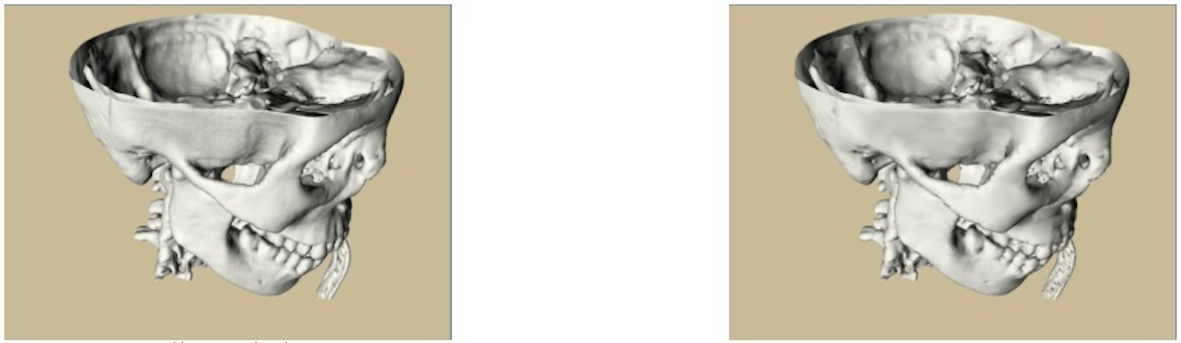
\includegraphics[width=0.85\textwidth]{dec_schroeder.jpg}
\caption{Example from the original paper, left full resolution (569k triangles) and right the 90\% decimated version (142k triangles) \citep[][p.68]{Schroeder1992}.}
\label{fig:dec_schroeder}
\end{figure} 

    \item Redistributing vertices over a surface \citep[cf.][]{Turk1992}.\\
The idea is to reduce the number of polygons by adding new points on the surface of the model, connecting these new vertices into triangles forming a mutual tessellation. Thus creating an intermediate polygonal surface that incorporates both the old vertices and the newly placed ones and then deleting the old vertices, i.e. re-tiling the surface. In order to maintain accurately the features of the surface, the point distribution is modified so that more new vertices are placed in regions of higher curvature (also see figure \ref{fig:dec_turk}).
%Bild
\begin{figure}[ht]
\centering
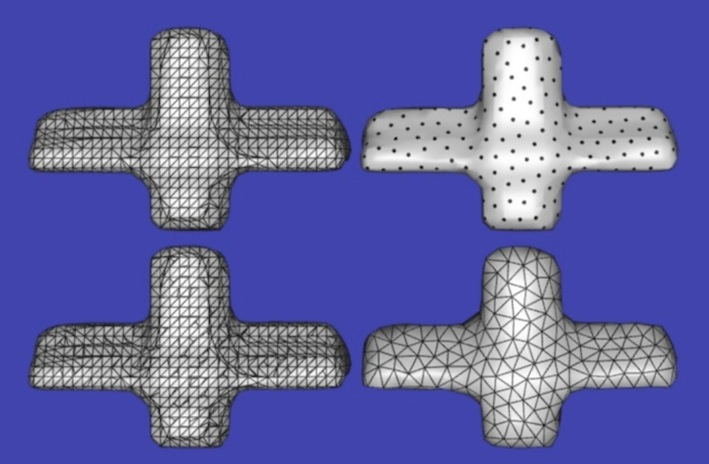
\includegraphics[width=0.50\textwidth]{dec_turk.jpg}
\caption{Re-tiling of a radiation iso-dose surface. Upper left: Original surface. Upper right: Candidate vertices after point-repulsion. Lower left: Mutual tessellation. Lower right: Final tessellation \citep[][p.58]{Turk1992}.}
\label{fig:dec_turk}
\end{figure} 

    \item Clustering vertices \citep[cf.][]{Rossignac1993}.\\
Is done by merging vertices based on their spatial proximity. All vertices within each cell of the subdivided 3D are collapsed into a single representative vertex for the voxel. Hence the resolution of the grid determines the level of detail achieved.
%Bild
\begin{figure}[ht]
\centering
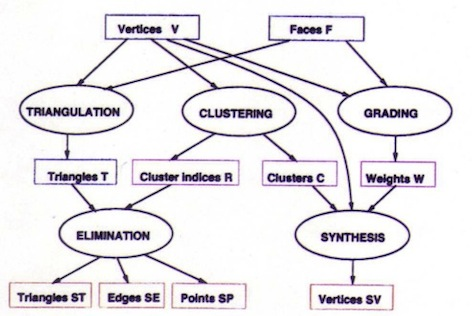
\includegraphics[width=0.60\textwidth]{dec_rossignac.jpg}
\caption{Overview of the simplification process \citep[][p.458]{Rossignac1993}.}
\label{fig:dec_rossignac}
\end{figure}
The algorithm is very robust as for it can deal with degenerated models and can also be implemented efficiently, but it is sensitive to the orientation of the clustering grid. Also, since topology is not preserved, it is very hard to give guaranteed explicit error bounds (also see figure \ref{fig:dec_rossignac}).

    \item Merging nearly coplanar polygons \citep[cf.][]{Hinker1993}.\\
This method obtains impressive reductions for large models with nearly flat surfaces. It identifying coplanar or nearly coplanar polygons, merging them together into a larger complex polygon and finally re-triangulating them into fewer polygons than the original description. However, this approach offers only small gains
for surfaces of high curvature (also see figure \ref{fig:dec_hinker}).
%Bild
\begin{figure}[ht]
\centering
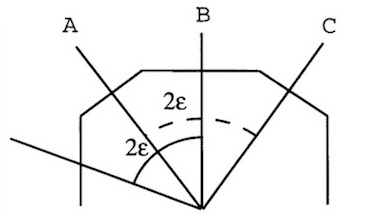
\includegraphics[width=0.30\textwidth]{dec_hinker.jpg}
\caption{
$2\epsilon$ is the user specified angle describing the maximum angular difference between coplanar sets selected to be merged \citep[][p.192]{Hinker1993}.}
\label{fig:dec_hinker}
\end{figure}

    \item Removing polygons in order of curvature \citep[cf.][]{Hamann1994}.\\
Given a surface triangulation, each triangle is weighted according to the principal curvature at its vertices.
These curvature values are pre-computed based on a parametric representation of the surface.
A triangle is associated with a surface region of low curvature if the sum of the absolute curvatures at its vertices is low.
The lower the curvature value at the vertices of a triangle the lower its weight.
The triangle with lowest weight is removed.
%Bild
\begin{figure}[ht]
\centering
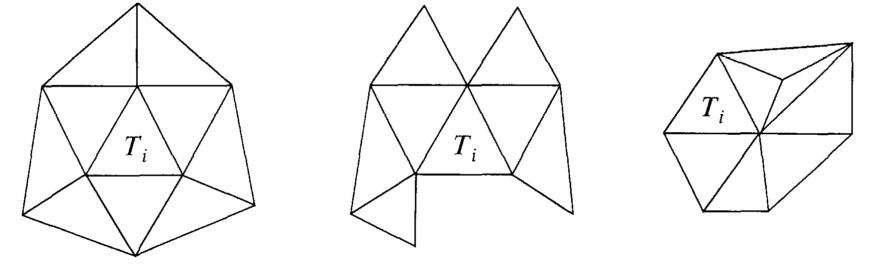
\includegraphics[width=0.75\textwidth]{dec_hamann.jpg}
\caption{The different cases for a triangle platelet $P_{i}$, i.e. the data stencil in the surface triangulation affected by the removal of triangle $T_{i}$ --  platelets with cyclic, disconnected and connected corona \citep[][p.200]{Hamann1994}.}
\label{fig:dec_hamann}
\end{figure}
The region affected by the removal is re-triangulated and new weights are computed for all affected triangles (also see figure \ref{fig:dec_hamann}).

    \item Using Wavelet theory \citep[cf.][]{Eck1995}.\\
A mesh is converted into a sample mesh together with a sequence of local correction terms, i.e. wavelet coefficients that capture the detail present in the model at various resolutions. The algorithm uses enough wavelet coefficients to meet a user specified error
bound. An important contribution of this method is that it overcomes subdivision connectivity restrictions. It constructs a continuous parametrization of an arbitrary mesh over a simple domain mesh, thus all arbitrary meshes can be converted to multiresolution form (also see figure \ref{fig:dec_eck}).
%Bild
\begin{figure}[ht]
\centering
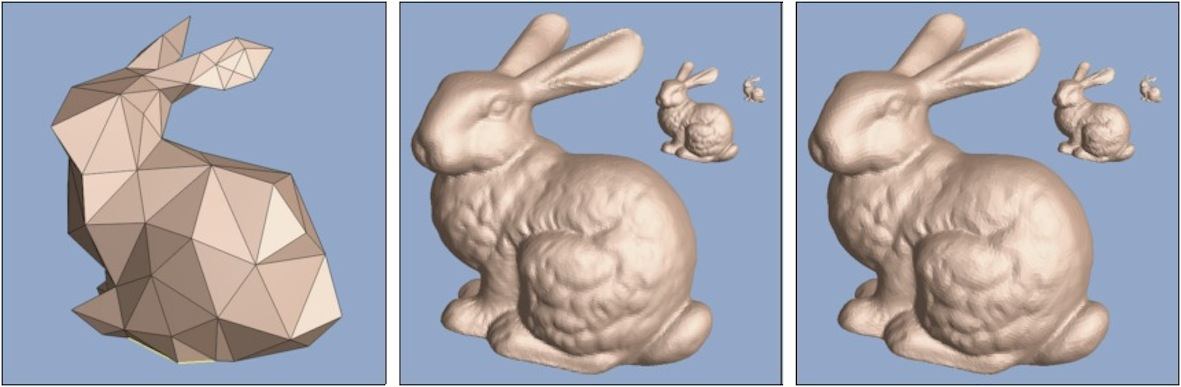
\includegraphics[width=0.80\textwidth]{dec_eck.jpg}
\caption{Left: Base mesh (162 triangles). Middle: Original mesh (69,437 triangles). LOD using multiresolution approximation \citep[][p.181]{Eck1995}.}
\label{fig:dec_eck}
\end{figure}

    \item Minimizing an energy function \citep[cf.][]{Hoppe1996}.\\
Hoppe presents a framework, called 'Progressive Meshes', which consist of a base mesh created by a sequence of edge collapses and vertex splits together with a sequence of detailed records that indicate how to incrementally refine the base mesh exactly back to the original mesh.
%Bild
\begin{figure}[ht]
\centering
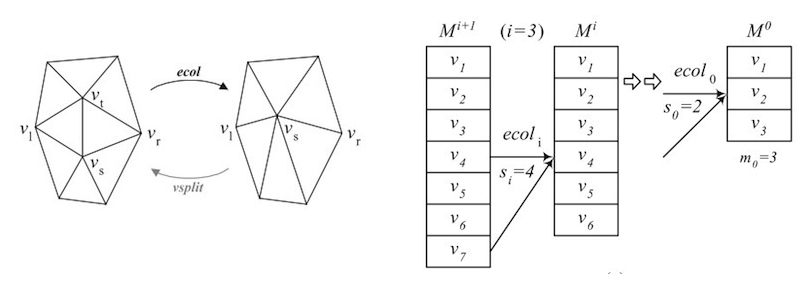
\includegraphics[width=0.90\textwidth]{dec_hoppe.jpg}
\caption{Original illustration of the edge collapse transformation respectively the vertex split and the resulting vertex correspondences \citep[][p.100]{Hoppe1996}.}
\label{fig:dec_hoppe}
\end{figure}
The sequence of collapses during a simplification is determined explicitly as an energy function to be minimized.
All edges to be collapsed are evaluated according to the energy function and sorted in a priority queue.
'Progressive Meshes' also introduced a very efficient data structure that can be used to represent a triangle mesh at multiple levels of detail, i.e. progressive refinement (also see figure \ref{fig:dec_hoppe}).
This techniques has been widely used for view-dependent simplifications, as well as progressive transmissions \citep[cf.][]{Bajaj1999}.

    \item Using bounding surfaces \citep[cf.][]{Cohen1996}.\\
A proposed method called “Simplification envelopes”.
The approach guarantees an error bound so that all points of an approximation are within a user-specifiable distance from the original model, also it enforces global and local topology preservation.
Simplification envelopes of a surface consists of two offset surfaces.
The outer and inner envelope are generated by displacing each vertex of the original mesh along its normal by a defined distance $\pm\epsilon$, which then guides the process.
A strong suit of this method is that it can gracefully deal with sharp edges (also see figure \ref{fig:dec_cohen}).
%Bild
\begin{figure}[ht]
\centering
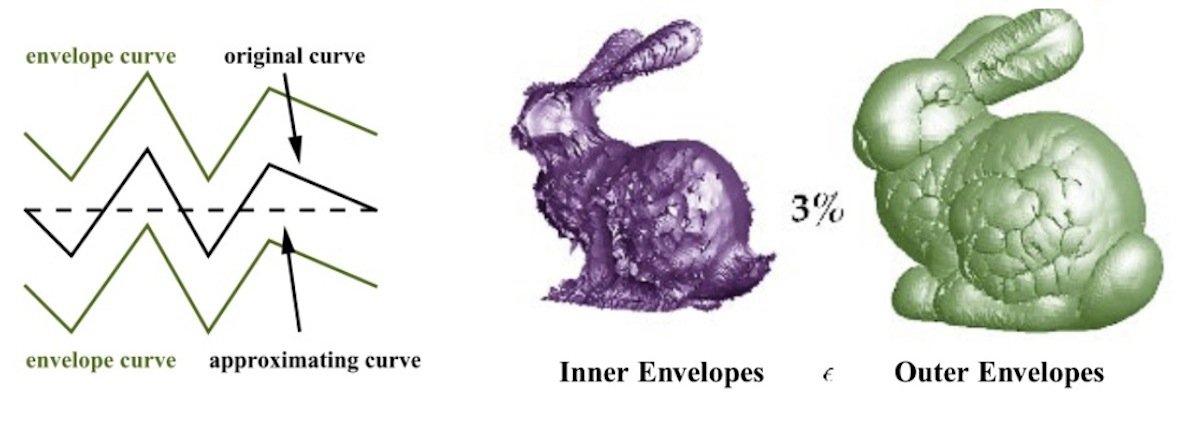
\includegraphics[width=0.80\textwidth]{dec_cohen.jpg}
\caption{Approximation with inner \& outer envelopes \citep[][pp.123-124]{Cohen1996}.}
\label{fig:dec_cohen}
\end{figure}

    \item Quadric Error Metrics \citep[cf.][]{Garland1997}.\\
The algorithm uses iterative contractions of vertex pairs to simplify models and maintains surface error approximations using quadric matrices.
By contracting arbitrary vertex pairs and not just edges, the algorithm can change the topology of the mesh and does it need a manifold mesh to begin with.
As the algorithm proceeds, a geometric error approximation is maintained at each vertex $\mathbf{v}$ of the decimated model: $\Delta(\mathbf{v})= \mathbf{v}^{T}\mathbf{Q}\mathbf{v}$, for a given contraction $(\mathbf{v_{1}},\mathbf{v_{2}}) \rightarrow \mathbf{v_{12}}$ the new matrix $\mathbf{Q_{12}}$ can be easily derived by simply adding $\mathbf{Q}_{1} + \mathbf{Q}_{2} = \mathbf{Q_{12}}$.
Simplification with quadric error metrics possesses much of the generality of vertex clustering as well as the quality and control of iterative contraction algorithms.
The only downside is its relative slowness compared to vertex clustering (also see figure \ref{fig:dec_garland}).
%Bild
\begin{figure}[ht]
\centering
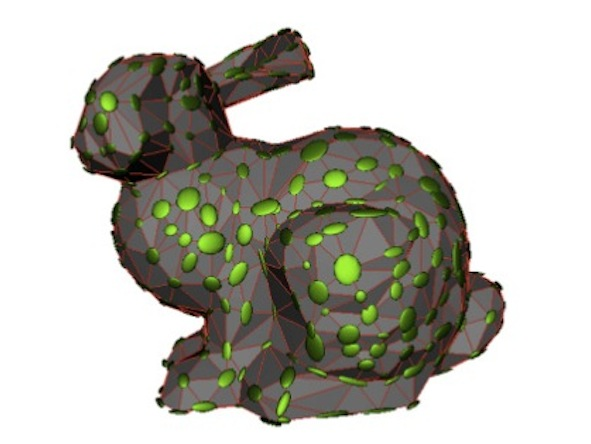
\includegraphics[width=0.50\textwidth]{dec_garland.jpg}
\caption{98,5\% decimation of the stanford bunny. The error ellipsoids for each vertex are shown in green \citep[][p.215]{Garland1997}.}
\label{fig:dec_garland}
\end{figure}

    \item Vertex placement for collapsed edges \citep[cf.][]{Lindstrom1998}.\\
Using edge collapse as the method for simplifying, edges are incrementally replaced with a single vertex.
The new vertex is placed so it preserves the location and shape, and does not require the retriangulation.
%Bild
\begin{figure}[ht]
\centering
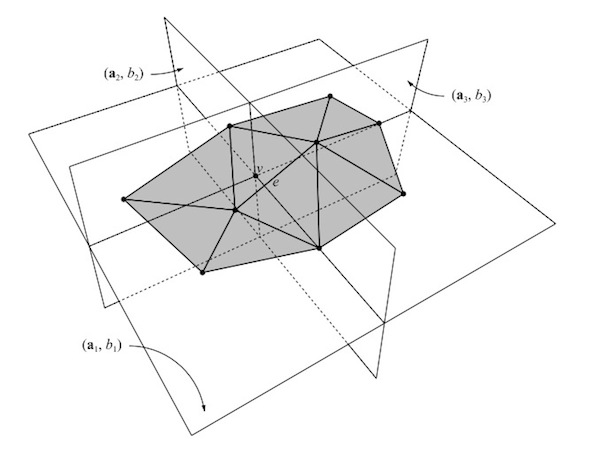
\includegraphics[width=0.50\textwidth]{dec_lindstrom.jpg}
\caption{The optimal vertex position $v$ expressed as the intersection of three planes that ensure volume preservation \citep[][p.284]{Lindstrom1998}.}
\label{fig:dec_lindstrom}
\end{figure}
The decision of how to position and order the edges builds upon volume and surface information.
Since these conditions do not fully determine the decimation process, an optimization stage is added.
Per triangle volume and area differences are used to create the priority queue (also see figure \ref{fig:dec_lindstrom}).

    \item Using image compression for geometry \citep[cf.][]{Gu2002}.\\
Most of the time surface geometry is modeled with irregular triangle meshes, i.e. not constant valency. In their paper, the authors devise a method to remesh an arbitrary surface onto a completely regular structure they call a geometry image. By this enabling them to represent geometry as a simple 2D array of quantized points. Surface signals like normals and colors are stored in similar 2D arrays using the same implicit surface parametrization. To create this geometry image, the mesh is cut along a network of edge paths, and the resulting single chart is parametrized onto a square\footnote{ More precisely the geometry is mapped onto a torus, since it is the only 3D manifold that can be a completely regular quad mesh and accordingly a regular triangle mesh with valence 6. With two cuts the torus then is equivalent to a 2D array (for a proof of this statement see Appendix \ref{appendix4}).}. The ingenious twist is, that in this form geometry images can be encoded using traditional lossy image compression algorithms, such as JPEG.
This is not so much a practical solution for mesh decimation as it is a striking example of how lifting one problem into another domain can lead to unexpected discoveries and new ideas (also see figure \ref{fig:dec_gu}).
%Bild
\begin{figure}[ht]
\centering
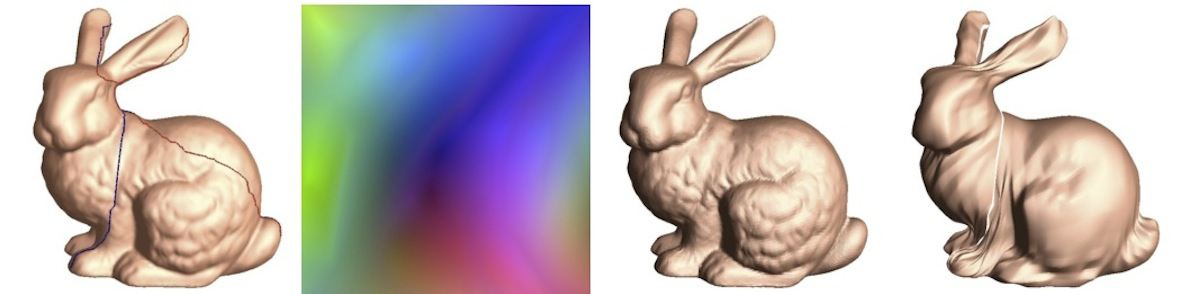
\includegraphics[width=1.0\textwidth]{dec_gu.jpg}
\caption{Left: Original mesh and its geometry image. Right: Reconstruction of original and a 1,5kB compressed mesh \citep[][p.356]{Gu2002}.}
\label{fig:dec_gu}
\end{figure}
\end{itemize}
This section can not give an exhaustive nor overall account of mesh simplification, but hopefully by example it illustrated the richness of the solutions and the progress already made.
The next section will try to bring together the various ideas presented here in order to give a general frame of reference, that is to say principles for taxonomies.

\newpage	
\section{Taxonomies}
\label{simplification3}

Besides listing important ideas and trying to get a feel for viable solutions, there is a second important step to get a firm grasp of a topic.
Namely by aggregating the ideas in question, grouping the similar ones and putting them into a relational structure, i.e. building a taxonomy.
This way, one does not only inductively broaden his knowledge one case at a time, but also deductively establish an overall framework for the principle problems in question.
Good taxonomies give the impression of necessity, as insofar as the taxa used to create the divides seem to be without alternatives, however some times at the cost of blocking the sight for alternatives\footnote{ It is worth mentioning that taxonomies are normally presented as prefaces to discussions of individual solutions. By doing this, the view on the actual evolution gets biased. Research is a fundamentally inductive endeavor. \begin{quote} \textit{``The view is often defended that sciences should be built up on clear and sharply defined basal concepts. In actual fact no science, not even the most exact, begins with such definitions. The true beginning of scientific activity consists rather in describing phenomena [and coming up with heuristics, only then] to group, classify and correlate them.''} \citep[cf.][]{Freud1963} \end{quote}.}.\\
Most taxonomies concerning mesh simplification, that can be found today, seem to be derived from the seminal work of Kobbelt \citep[][cf. p.6]{Gotsman2002}.
As it were, the prototypical taxonomy is as follows \citep[][cf. p.11]{Shene2005}:
\begin{itemize}
  \setlength{\itemsep}{0cm}%
  \setlength{\parskip}{0cm}%
    \item \textbf{Vertex Clustering} -- Usually very efficient, robust and the complexity is typically linear: $\mathbf{O}(|\mathcal{V}|)$, where $|\mathcal{V}|$ is the number of vertices. However, the quality of the resulting mesh is not always satisfactory.\\
    \item \textbf{Incremental Decimation} -- Delivers higher quality meshes in most cases and can take arbitrary user-defined criteria into account, according to how the next removal operation is chosen. Though, complexity is normally higher: $\mathbf{O}(|\mathcal{V}| \log_{2} |\mathcal{V}|)$, and can go up to $\mathbf{O}(|\mathcal{V}|^{2})$ especially when a global threshold has to be met.\\
    \item \textbf{Resampling} -- Most general approach. The major motivation for building a completely new mesh is to maintain a special connectivity structure like subdivision connectivity. Problematic is its higher proneness to alias errors.\\
\end{itemize}
The three cases are obviously very broad and each of them can be further characterized by classifying more details.
For example could 'Vertex Clustering' algorithms be sorted whether they apply a hierarchical or top-down approach, or how they compute representative vertices: average, median, error quadrics and so forth.
Likewise 'Incremental Decimation' algorithms can be organized by the decimation operators they use: Topology-changing vs. topology-preserving, subsampling vs. filtering, existence of inverse operations, etc. -- for an exhaustive discussion of these aspects, we recommend the paper ``A General Framework for Mesh Decimation'' \citep[cf.][]{Kobbelt1998}.

The standard taxonomy is practical and easy to understand but it does not seem to follow any specific principle or foundation.
This is especially obvious when confronted with algorithms that overstep the traditional scheme -- such as probabilistic optimization techniques of multiple-choice algorithms \citep[cf.][]{Wu2002}, or the 'TopStoc' algorithm that will be discussed in detail later \citep[][cf.]{Boubekeur2009}.
\begin{table}[htpb]
\medskip
\setlength{\tabcolsep}{15pt}
\renewcommand{\arraystretch}{1.5}
   \centering
\begin{tabular}{ l || c | c } \centering
    & \textbf{Clustering} & \textbf{Incremental} \\ \hline \hline
  \textbf{Deterministic} & Spatial clustering & Priority queue \\
  \textbf{Stochastic} & TopStoc & Multiple choice \\
\end{tabular}
   \label{tab:taxonomies} \medskip
   \caption{Taxonomy from Boubekeur \& Alexa \citep[p.2]{Boubekeur2009}.}
\end{table}\\
A more general classification can be set up when comparing mesh simplification to a method from signal processing, that is, vector quantization.
Vector quantization has traditionally been used for lossy data compression, but has also applications for lossy data correction and density estimation.
The following description adopts the ideas described in the paper ``Model Simplification Through Refinement'', which first made the argument of familiarity \citep[][cf. pp.221-222]{Brodsky2000}:\\
Vector quantization is the process of mapping a vector in a large set $\mathcal{S} \subset \mathbb{R}^{n}$ into a smaller set $\mathcal{T} \subset \mathbb{R}^{n}$ with $\mathcal{T}$ partitioning the set $\mathcal{S}$, hence $|\mathcal{S}| > |\mathcal{T}|$.
This is done by a so called quantizer function $\mathcal{Q}: \mathbb{R}^{n} \rightarrow \mathcal{T}$.
Where $\mathcal{T} = \{\vec{v}_{i} \in \mathbb{R}^{n} | 1 \leq i \leq N\}$ represents all vectors in $\mathcal{S} \subset \mathbb{R}^{n}$.
The goal is to find the best $\mathcal{T}$ to represent all vectors in $\mathcal{S}$.
When the distortion between an input vector is minimal for all $\vec{v} \in \mathcal{S}$, then $\mathcal{T}$ is called optimal.\\
This definition looks familiar to the one given at the beginning of the chapter \ref{simplification1}, with: $\mathcal{S} \propto \mathcal{M}$ the base mesh, and $\mathcal{T} \propto \mathcal{M'}$ the decimated mesh, respectively $\mathcal{Q}$ representing a decimation algorithm.\\
Gersho and Gray list the four basic types for vector quantization algorithms \citep[][cf. pp.358 ff.]{Gersho1991}:
\begin{enumerate}
	\item So called \textbf{'product code'} algorithms use scalar quantizers that are independently applied to each input vector element.
	The main difference to other methods is, that the partitioning set $\mathcal{T}$ is built once and not iterated upon.\\
	An analogy for these type are clustering algorithms, where partitions are formed with a uniform voxelization.	
	\item  In \textbf{'pruning algorithms'}, $\mathcal{T}$ initially contains all the vectors of the input set $\mathcal{S}$. The entry $\vec{v}_{mindis} \in \mathcal{T}$ that increases distortion least is removed and removals continue until the desired size of $\mathcal{T}$ reached.\\
	Simplification algorithms taking the pruning approach are for instance algorithms, that growing coplanar patches, or that remove and pruning away single vertices.
	\item Pairwise \textbf{'nearest neighbor'} algorithms also set $\mathcal{T}$ to contain all the vectors in $\mathcal{S}$. All possible pairs $(\vec{v}_{i},\vec{v}_{j}) \in \mathcal{T} \text{ with } i\neq j$ are considered and the pair that introduces the least distortion is merged. Merging continues until the desired size for $\mathcal{T}$ or distortion tolerance is reached.\\
	Vertex merge or edge collapse algorithms are of this kind. They merge the vertices, recompute the affected vertex pairs, and iterate.
	\item In \textbf{'splitting algorithms'}, $\mathcal{T}$ initially contains a single partition of $\mathcal{S}$. The partition with the most distortion is located and then split. Splitting continues until the required distortion or size is reached.\\
	Only very few actual decimation techniques use this quasi inverse method of starting with a base primitive and then adaptively subdividing it until the desired decimation level is reached.
\end{enumerate}
In other words, the logic of the classification is to look at possible dynamics for partitioning, since there are just three principle ways to form $\mathcal{T}$: One can sets it statically (\textbf{'product code'}), or produce it step by step, either via a top-down (\textbf{'pruning algorithms'} and \textbf{'nearest neighbor'}) or bottom-up approach (\textbf{'splitting algorithms'}).

Besides having a complete taxonomy, the last point to discuss is, upon which differentiations any simplification algorithm should be distinguished and designed.
We compiled the following checklist to lists the most important attributes to characterize any mesh decimation algorithm and thus are also the question one should answer before implementing any code:
\begin{table}[htb]
\medskip
\setlength{\tabcolsep}{10pt}
\renewcommand{\arraystretch}{1.5}
   \centering
\begin{tabular}{ l l c r } \centering
	The decimation process is \dots & \textbf{automated} & $\longleftrightarrow$ & \textbf{with user input} \\
	The result is measured \dots & \textbf{perceptual} & $\longleftrightarrow$ & \textbf{analytical} \\
	The algorithm works \dots & \textbf{deterministic} & $\longleftrightarrow$ & \textbf{stochastic} \\
		 & \textbf{incremental} & $\longleftrightarrow$ & \textbf{static} \\
 	The input data is \dots \dots & \textbf{constrained} & $\longleftrightarrow$ & \textbf{arbitrary} \\
	\dots~ and must be topologically \dots & \textbf{transformed} & $\longleftrightarrow$ & \textbf{preserved} \\
	The work-flow regime is \dots & \textbf{off-line} & $\longleftrightarrow$ & \textbf{realtime} \\
\end{tabular}
   \label{tab:check_list} \bigskip
   \caption{Checklist for simplification algorithms.}
\end{table}\\
We have ordered the checklist in so far, as the the work presented in this thesis, aims to meet the description on the right hand side of table \ref{tab:check_list}: We introduce a very fast, user-guided decimation algorithm with topology control, that can handle non-manifold triangle meshes.
In addition to that, our approach addresses a number of problems that are pivotal for a practical solution: Texture handling, point of view decimation, reproducibility, etc. 

Before describing the details of our solution and discussing the results we achieved, the next chapter \ref{math0} will set a solid mathematical foundation for describing the topological challenges we encountered during our work.
